% 第 20 题椭圆图：按固定源内容流矢量层精确值复刻（1 pt → 0.03515 cm，与全库同制）。
% 原点取 x 轴负端 x=616.6363 pt、y 轴下端 y（顶向下）=301.4517 pt；y 向上（Y = 301.4517 − y_页）。
% 源实测（figure-inventory §5）：中心 O=(76.5367,56.6933)、半轴 a=56.6933 / b=40.0815，a/b=1.414451≈√2；
%   椭圆线宽 0.79701bp（其余线的 2 倍，全卷唯一加粗线——突出二次曲线，照源）；x 轴、y 轴、割线线宽 0.3985；
%   4 段三次贝塞尔闭合，控制点偏移比 0.55225(x)/0.55231(y)≈0.55228，本图用 TikZ ellipse 同制。
%   作图比例尺 1 cm = 1 单位（a=2.00000 cm、b=1.41435 cm），椭圆即 x²/4+y²/2=1（题干 (1) 的答案）。
%   x 轴自左端过中心向右，线段末端 149.4861、箭尖 153.0734（至左端左右对称外伸 19.8434）；
%   y 轴自下端过中心向上，线段上端 112.6324、箭尖 116.2197（上端外伸 19.4449）；两箭头为源内纯填充三角（2.9894×3.9859）。
%   全图 3 直线段 + 1 椭圆 + 2 枚箭头，无虚线、无区域填充、无点标记；标签 6 个（x、y、A、B、P、O），
%   照源字形盒中心定位；图上不标椭圆顶点与焦点。
% 源内异常（照源复刻、已登记，见 §5.3 E-1）：割线 l 实测端点 (13.4933,37.7056)–(104.3128,108.6973)、
%   长 115.2899、斜率 −0.781676，与 y 轴交点 y=1.0686 单位 ≠ 题干 P(0,1) 的 1.0000（差 1.946 pt），
%   且为两端伸出椭圆外的延长割线。**此处照源实测端点抄录，勿按题干「修正」为过 (0,1)**。
% 注：本注释内坐标均为本图坐标系（X = x_页 − 616.6363，Y = 301.4517 − y_页），与代码逐值一致。
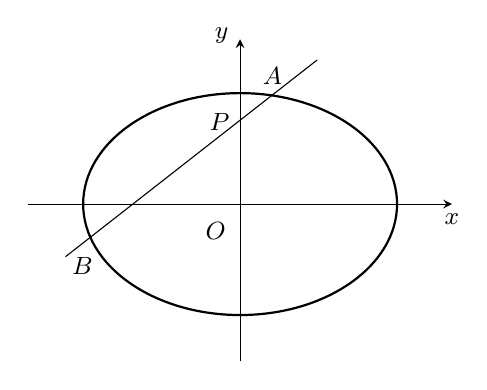
\begin{tikzpicture}[x=0.03515cm,y=0.03515cm,>=stealth,every node/.style={font=\small,inner sep=0pt}]
% ===== 椭圆（4 段贝塞尔，线宽 0.79701 为全卷唯一加粗）=====
\draw[line width=0.79701bp] (76.5367,56.6933) ellipse [x radius=56.6933, y radius=40.0815];
% ===== 两轴与箭头（照源：直线段 + 独立填充三角，此处并入线端）=====
\draw[line width=0.3985bp] (0,56.6933)--(149.4861,56.6933);           % x 轴（线段，右端）
\draw[->,line width=0.3985bp] (149.4861,56.6933)--(153.0734,56.6933); % x 轴箭头（尖端照源）
\draw[line width=0.3985bp] (76.5367,0)--(76.5367,112.6324);           % y 轴（线段，上端）
\draw[->,line width=0.3985bp] (76.5367,112.6324)--(76.5367,116.2197); % y 轴箭头（尖端照源）
% ===== 割线 l（过 P 的动直线；照源实测端点，两端伸出椭圆外）=====
\draw[line width=0.3985bp] (13.4933,37.7056)--(104.3128,108.6973);
% ===== 标签 6 个（照源字形盒中心定位）=====
\node at (69.8847,117.6067) {\(y\)};
\node at (88.2192,103.1367) {\(A\)};
\node at (69.0962,86.1807) {\(P\)};
\node at (67.6922,47.0137) {\(O\)};
\node at (19.5517,34.4447) {\(B\)};
\node at (153.0712,51.0977) {\(x\)};
\end{tikzpicture}
